\section{Development \& Results}
\begin{frame}{Development \& Results}
Development is divided into:
\begin{itemize}
    \item EEG MI Classifier
    \item Dataset Augmentation Technique
    \item Virtual Environment
    \item Project Testing Pipeline
\end{itemize}
\end{frame}

\begin{frame}{EEG MI Classifier - Baseline Methods}
    \begin{minipage}[c]{.65\textwidth}
        \begin{itemize}
            \item \textbf{CSP + LDA}: Common Spatial Patterns + Linear Discriminant Analysis
            \item \textbf{TGSP + SVM}: Tangent Space Projection + Support Vector Machine
            \item \textbf{MDM}: Minimum Distance Mean
            \item \textbf{EEGNetV4}: Convolutional Neural Network for Motor Imagery Classification
        \end{itemize}        
    \end{minipage}
    \begin{minipage}[c]{.33\textwidth}
        \begin{figure}[htpb!]
            \centering
            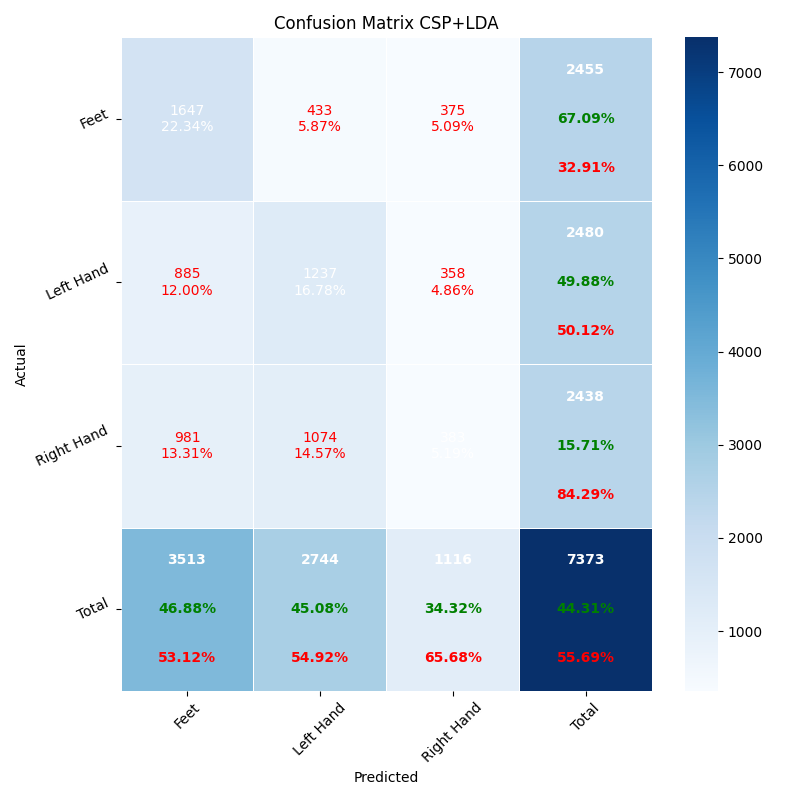
\includegraphics[width=0.45\textwidth]{figures/classification/confusion_matrix_csp_lda}
            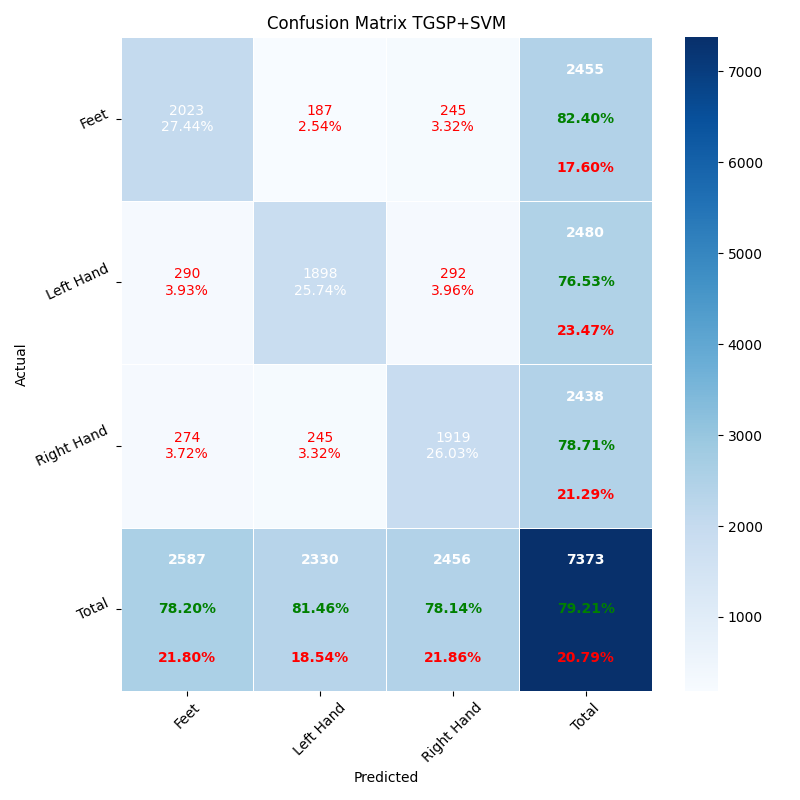
\includegraphics[width=0.45\textwidth]{figures/classification/confusion_matrix_tgsp_svm}
            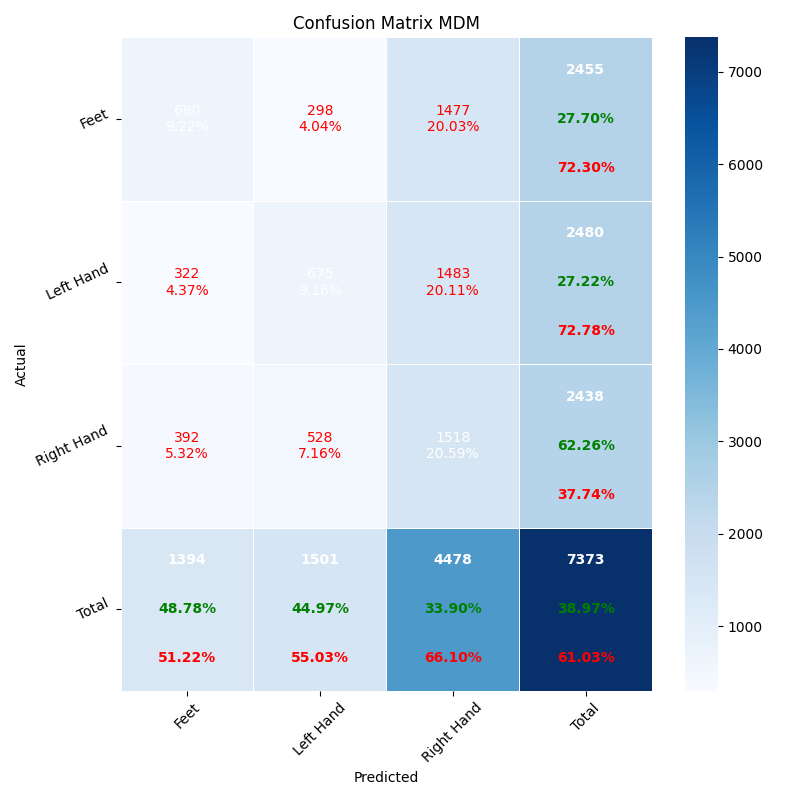
\includegraphics[width=0.45\textwidth]{figures/classification/confusion_matrix_mdm}\\
            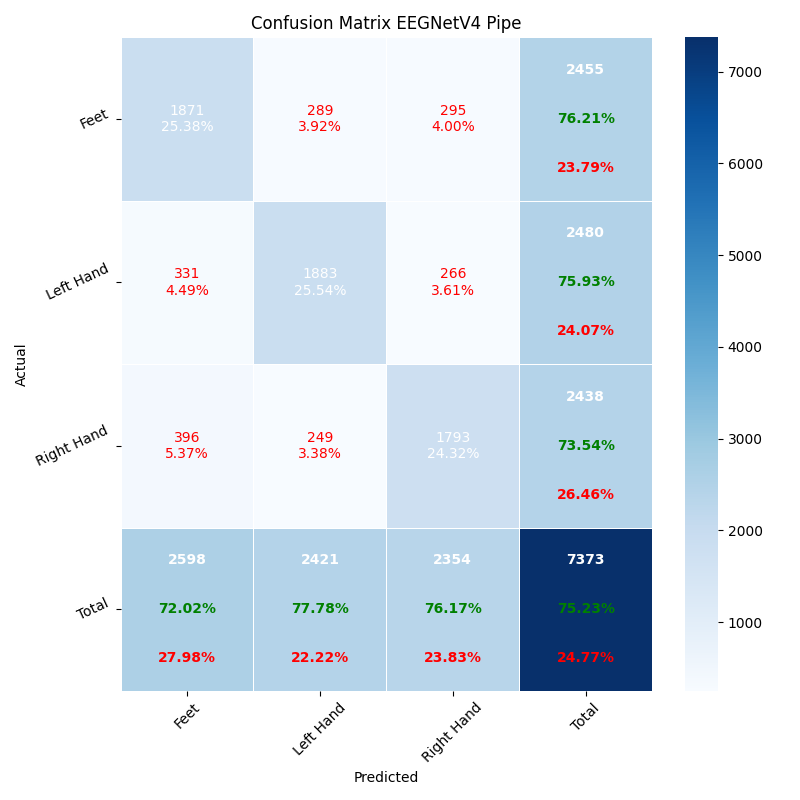
\includegraphics[width=0.45\textwidth]{figures/classification/confusion_matrix_eegnetv4_pipe}
            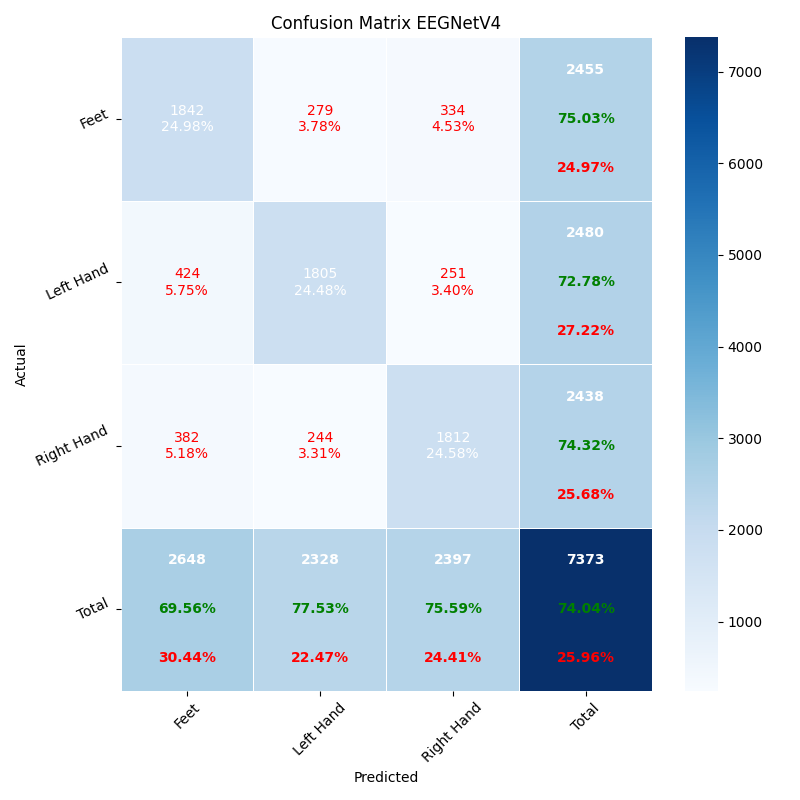
\includegraphics[width=0.45\textwidth]{figures/classification/confusion_matrix_eegnetv4}
        \end{figure}
    \end{minipage}
\end{frame}

\begin{frame}{EEG MI Classifier - Proposed Method}
    \begin{minipage}[c]{.65\textwidth}
        From ``\textbf{Deep temporal networks for EEG-based motor imagery recognition.}'' by \textit{Sharma N. et al.} (2023) I used and adapted: 
        \begin{itemize}
            \item LSTM-based Approach
            \item Transformer-based Approach
        \end{itemize}
    \end{minipage}
    \begin{minipage}[c]{.33\textwidth}
        \begin{figure}[htpb!]
            \centering
            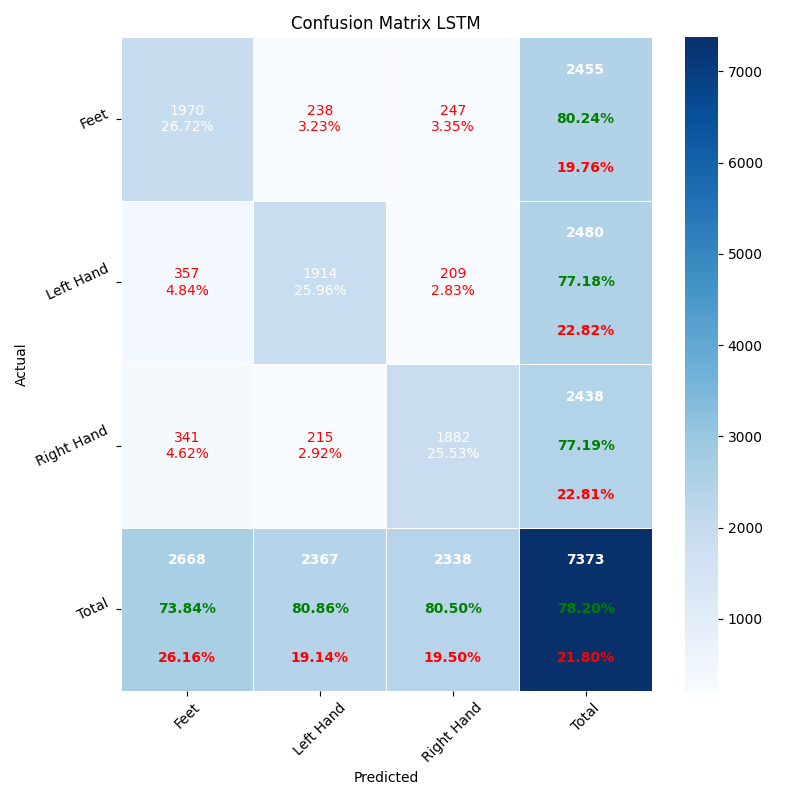
\includegraphics[width=\textwidth]{figures/classification/confusion_matrix_lstm}
            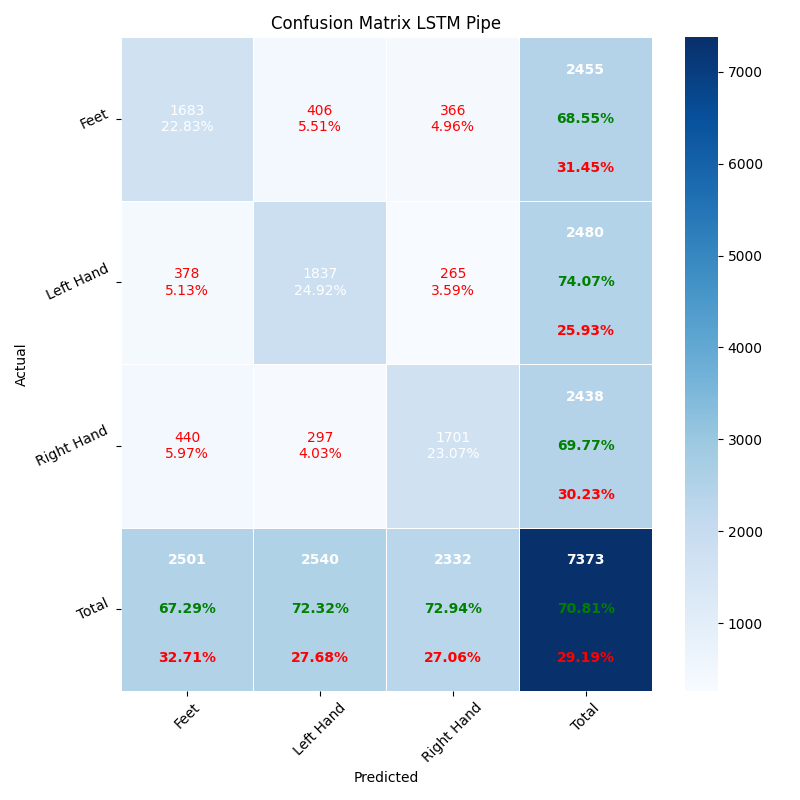
\includegraphics[width=\textwidth]{figures/classification/confusion_matrix_lstm_pipe}
        \end{figure}
    \end{minipage}
\end{frame}

\begin{frame}{Dataset Augmentation - GAN Based}
    \begin{minipage}[c]{.65\textwidth}
        From ``\textbf{EEGFuseNet: Hybrid Unsupervised Deep Feature Characterization and Fusion for High-Dimensional EEG With an \#Application to Emotion Recognition.}'' by \textit{Z. Liang et al.} (2021) I used and trained the network:
        \begin{itemize}
            \item GAN based Approach $\rightarrow{}$ EEGFuseNet
        \end{itemize}
    \end{minipage}
    \begin{minipage}[c]{.33\textwidth}
        \begin{figure}[htpb!]
            \centering
            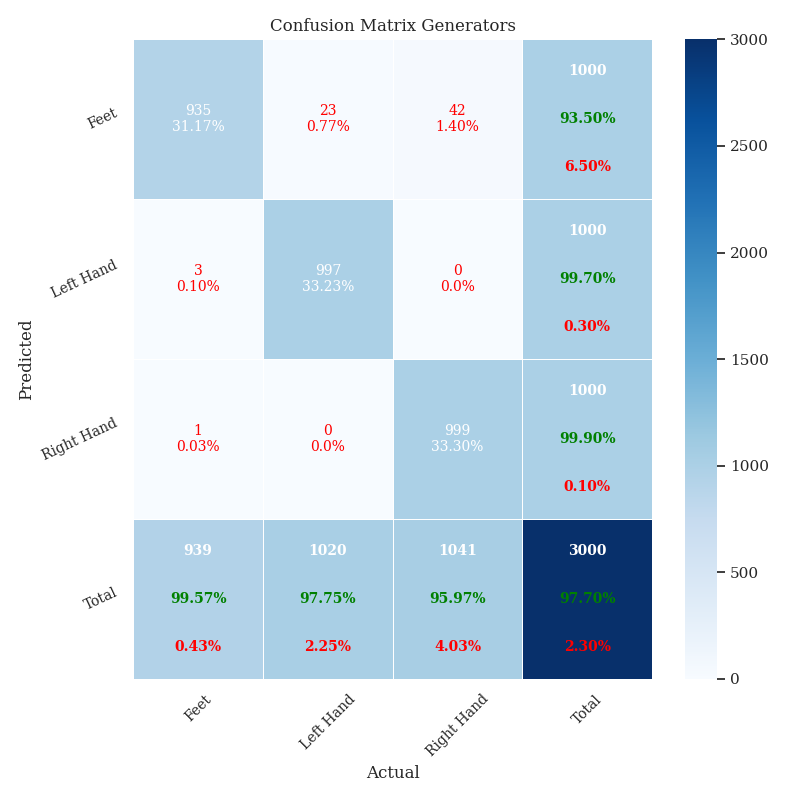
\includegraphics[width=\textwidth]{figures/augmentation/gan/confusion_matrix_generators_generators_using_LSTMNet_0.5943600867678959.pkl}
        \end{figure}
    \end{minipage}
\end{frame}

\begin{frame}{Dataset Augmentation - Stochastic Methods}
    \begin{minipage}[c]{.65\textwidth}            
        From ``\textbf{Data Augmentation for Deep Neural Networks Model in EEG Classification Task: A Review}'' by \textit{C. He et al} (2021) I created a script to generate data using:
        \begin{itemize}
            \item Stochastic Noise Injection Approach $\rightarrow{}$ Good Results
            \item Stochastic Generation Approach $\rightarrow{}$ Bad Results
        \end{itemize}
    \end{minipage}
    \begin{minipage}[c]{.33\textwidth}
            \centering
            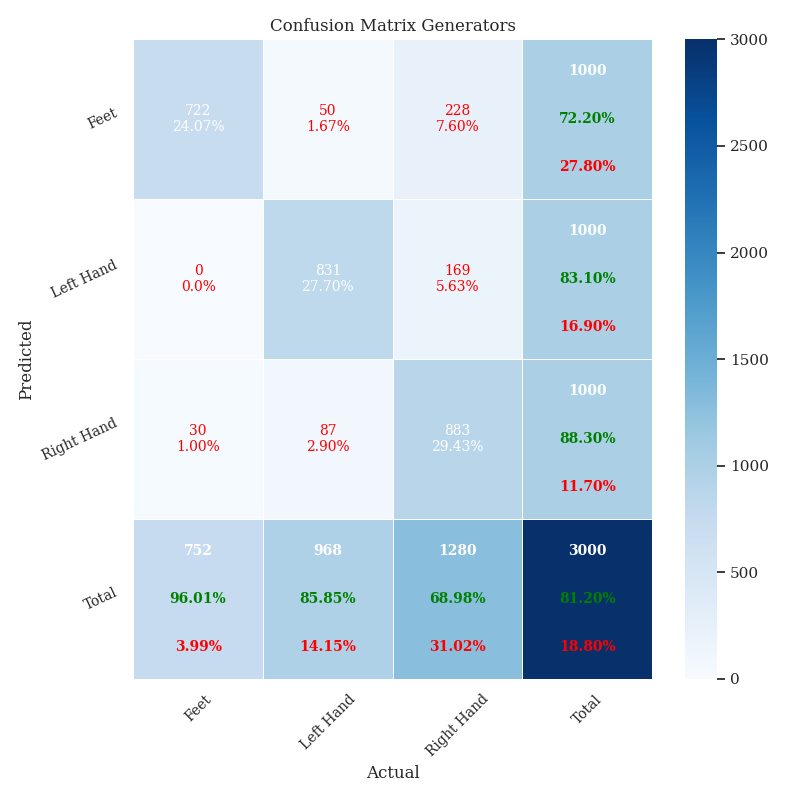
\includegraphics[width=.8\textwidth]{figures/augmentation/stochastic/confusion_matrix_generators_2024_03_30_18_00_20_noise_injector_using_LSTMNet_0.5943600867678959.pkl.png}\\
            {\tiny Noise Injection}\\
            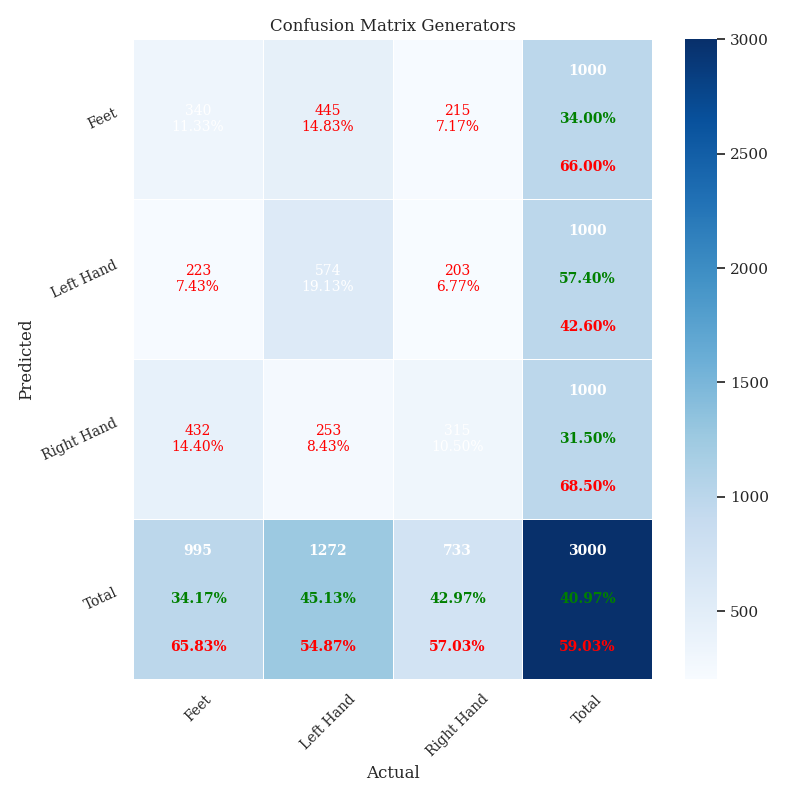
\includegraphics[width=.8\textwidth]{figures/augmentation/stochastic/confusion_matrix_generators_2024_03_30_18_01_19_random_sampler_using_LSTMNet_0.5943600867678959.pkl.png}
            {\tiny Random Sampling}
    \end{minipage}
\end{frame}

\begin{frame}{Project Testing Pipeline}
    \begin{minipage}[c]{.65\textwidth}
        \begin{itemize}
            \item Keyboard Controls (W/Space, A, D)
            \item EEG Signals Generation (Feet, Left Hand, Right Hand)
            \item Signal Classification
            \item Classification Transmission (Via WebSocket)
            \item Virtual Character Control
        \end{itemize}
    \end{minipage}
    \begin{minipage}[c]{.33\textwidth}
        \begin{figure}[htpb!]
            \centering
            \href{https://youtu.be/13iwuG1pyk0}{%
            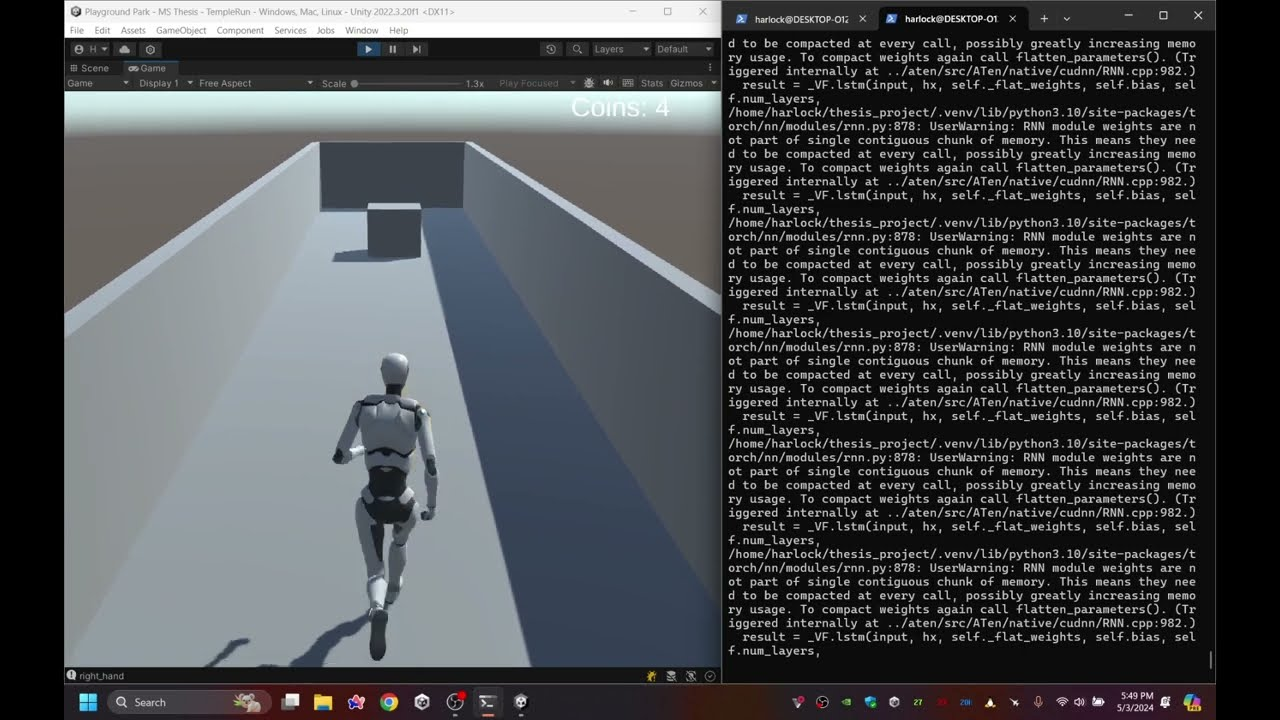
\includegraphics[width=\textwidth]{figures/gameplay/infinite_runner}%
            }
        \end{figure}
        \begin{figure}[htpb!]
            \centering
            \href{https://youtu.be/aBgP87yz1Lw}{%
            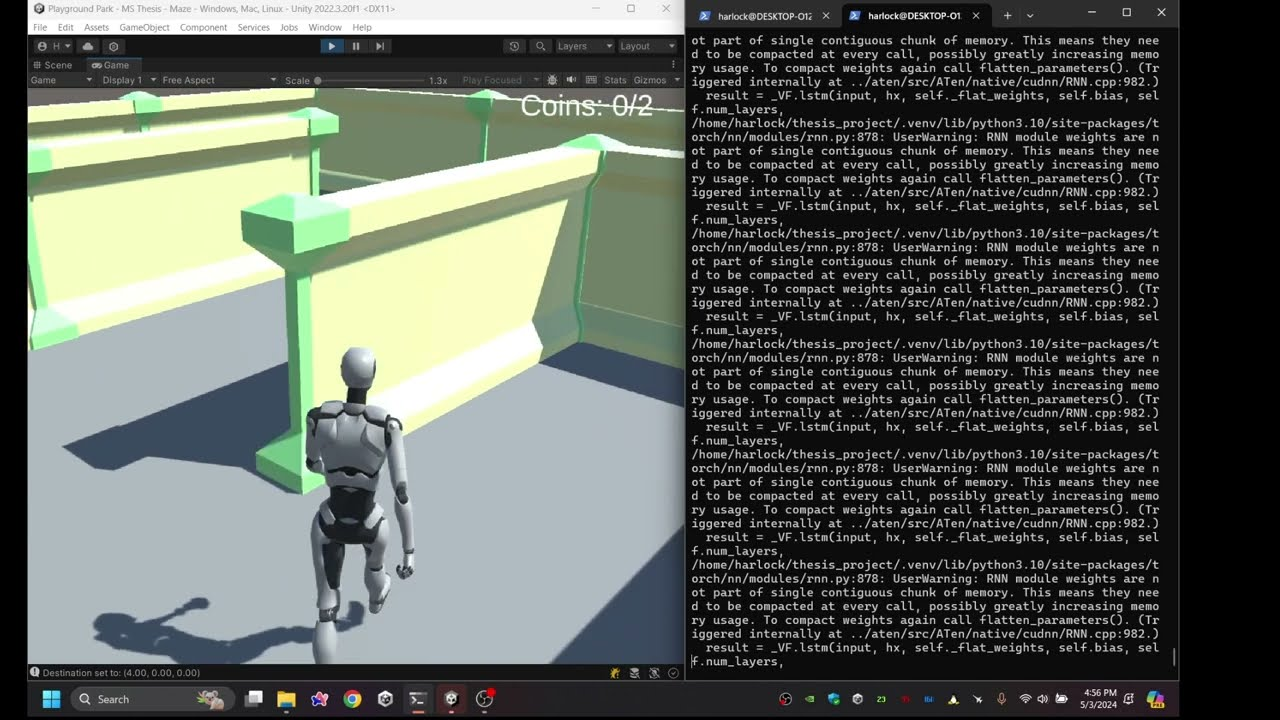
\includegraphics[width=\textwidth]{figures/gameplay/maze}%
            }
        \end{figure}
    \end{minipage}
\end{frame}